\section{Q-Learning-Experimente}

Um nun zu testen, ob die Landschaft für unsere Zwecke geeignet ist, werden wir einige Experimente durchführen. Wir wollen hierfür zunächst einen simplen Reinforcement-Learning-Agenten implementieren, welcher \textit{Q-Learning} verwendet.

\subsection{Das Prinzip von Q-Learning}
% \citeauthor{}

Dieses Kapitel stützt sich zu einem Großteil auf das Buch \textit{Reinforcement Learning: An Introduction, Second Edition} \cite{06_sutton2018reinforcement}. Falls nicht anders angegeben, wurden die Informationen hieraus entnommen.

\paragraph{Markov Decision Processes}
Alle folgenden Experimente zielen darauf ab, Probleminstanzen von \textit{Markov Decision Processes} -- oder kurz MDPs -- zu lösen. In MDPs gibt es eine handelnde Instanz, den \textit{Agenten}, welcher mit seinem Umfeld, der so genannten \textit{Umgebung} interagiert. Diese Interaktion erfolgt Sequenziell in Zeitschritten $ t = 0, 1, 2, 3, ... $. Der Agent erhält in jedem Zeitschritt $ t $ eine Repräsentation seiner Umgebung, den Zustand $ S_t $, und führt basierend darauf eine \textit{Aktion} $ A_t $ aus. Für diese erhält er von der Umgebung eine Belohnung $ R_{t + 1} $, sowie einen Folgezustand $ S_{t + 1} $.

\begin{figure}[H]
    \centering
    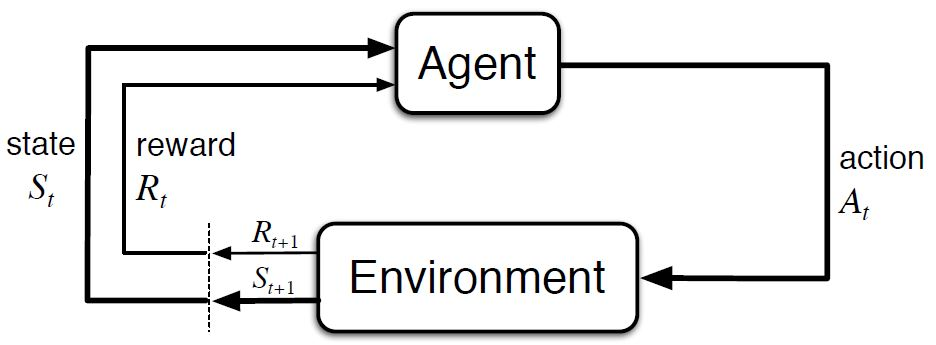
\includegraphics[width=0.5\textwidth, keepaspectratio=true]{mdp.JPG}
    \caption{Interaktion zwischen Umgebung und Agent in einem MDP} \label{img:mdp}
    \source{\cite{06_sutton2018reinforcement}}
\end{figure}

Ziel des Agenten ist es nun, seinen erwarteten Ertrag $ G_t $ zu maximieren. Im einfachsten Fall ist dieser die Summe aller Belohnungen:
\begin{align}
    G_t \doteq R_{t + 1} + R_{t + 2} + R_{t + 3} + ... + R_T \text{,} \label{eq:expected_reward}
\end{align}
wobei T Zeitschritt einer Episode ist. In vielen Fällen ist die Interaktion zwischen Agent und Umgebung allerdings nicht endlich. Somit ist in diesen Fällen $ T = \infty $ und der Ertrag, den der Agent maximieren soll, nach \ref{eq:expected_reward} unendlich. Wir führen deswegen das \textit{discounting} ein. Für $ G_t $ ergibt sich hiermit:
\begin{align}
    \begin{split}
        G_t & \doteq R_{t + 1} + \gamma R_{t + 2} + \gamma^2 R_{t + 3} + ...\\
        & = \sum_{k = 0}^{T} \gamma^k R_{t + k + 1} \text{,}
    \end{split} \label{eq:expected_discounted_reward}
\end{align}
wobei die \textit{discount rate} $ \gamma $ ein Wert zwischen $ 0 $ und $ 1 $ ist. Eine Belohnung $ k $ Zeitschritte in der Zukunft ist also nur $ \gamma^{k - 1} $--mal so viel wert wie eine Belohnung, welche im aktuellen Zeitschritt erhalten wurde.

\paragraph{Policies}
Der Agent folgt zu jedem Zeitpunkt einer Policy $ \pi $. Hierbei gibt $ \pi(a|s) $ die Wahrscheinlichkeit dafür an, dass der Agent zum Zeitschritt $ t $ die Aktion $ a \in A $ im Zustand $ s \in S $ ausführt, also dass die Aktion $ A_t = a $ wenn $ S_t = s $. Hierbei ist $ S $ die Menge aller Zustände und $ A $ die Menge aller Aktionen. $ \pi(a|s) $ ist also eine Wahrscheinlichkeitsverteilung über $ a \in A(s) $ für jedes $ s \in S $, wobei $ A(s) $ alle möglichen Aktionen im Zustand $ s $ beschreibt.

\paragraph{State-Value Functions}
Wir benötigen nun eine Möglichkeit einzuschätzen, wie gut ein Zustand $ s $ ist, wenn wir der Policy $ \pi $ folgen. Hierfür nutzen wir die \textit{state-value function} $ v_\pi $. Diese beschreibt die erwartete Belohnung eines Zustands $ s $ unter der Policy $ \pi $ zum Zeitschritt $ t $. Wir definieren $ v_\pi(s) $ als
\begin{align}
    \begin{split}
    v_\pi(s) & \doteq E_\pi \left[G_t | S_t = s \right]\\
    & = E_\pi \left[\sum_{k = 0}^{\infty} \gamma^k R_{t + k + 1} | S_t = s \right],
    \end{split}
\end{align}
wobei $ E_\pi $ der Erwartungswert des Ertrags $ G_t $ nach \ref{eq:expected_discounted_reward} ist, wenn der Agent sich im Zustand $ S_t = s $ befindet und der Policy $ \pi $ folgt.

\paragraph{Action-Value Functions}
Ähnlich hierzu gibt die \textit{action-value function} $ q_\pi $ an, wie profitabel es für den Agenten ist, in einem gegebenen Zustand eine gewisse Aktion auszuführen, wenn der Agent der Policy $ \pi $ folgt.

Der Wert einer Aktion $ a $ im Zustand $ s $ unter der Policy $ \pi $ ist also die erwartete Belohnung, wenn man im Zustand $ s $ zum Zeitschritt $ t $ die Aktion $ a $ ausführt. Wir definieren $ q_\pi(s, a) $ als
\begin{align}
    \begin{split}
    q_\pi(s,a) & \doteq E_\pi \left[G_t | S_t = s, A_t = a \right]\\
    & = E_\pi \left[\sum_{k = 0}^{\infty} \gamma^k R_{t + k + 1} | S_t = s, A_t = a \right].
    \end{split}
\end{align}
Die action-value function wird auch als Q-function bezeichnet, welche als Ergebnis für ein state-action Paar die Q-value liefert. Für die folgenden Implementierungen ist diese von großer Wichtigkeit.

\paragraph{Optimale Policies und Optimale Value Functions}
Das Ziel des Agenten ist, die optimale Policy $ \pi $ für ein Markov Decision Problem zu finden. Ist dieses Ziel erreicht so lässt sich sagen, dass die Reinforcement Learning Aufgabe erfüllt ist. Optimal ist hierbei die Policy, welche nach Aufsummieren der Belohnungen über alle Schritte einer Episode die beste gesamte Belohnung liefert. Eine Policy $ \pi $ ist also besser als Policy $ \pi' $, wenn die erwartete Belohnung von $ \pi $ für \textbf{alle} Zustände $ s \in S $ größer ist als die von $ \pi' $. \cite{06_sutton2018reinforcement} verwendet die Formulierung
\begin{align}
    \pi \geq \pi' \text{ if and only if } v_\pi(s) \geq v_{\pi'}(s) \text{ for all } s \in S.
\end{align}

Es gibt immer eine Policy, die besser als oder gleichwertig mit allen anderen Policies ist. Diese wird beziehungsweise werden als $ \pi_* $ bezeichnet. Die besten Policies besitzen die gleich state-value function, welche die \textit{optimale state-value function} $ v_* $ genannt wird und definiert wird als
\begin{align}
    v_*(s) \doteq \max_\pi v_\pi(s)
\end{align}
für alle $ s \in S $.

Optimale Policies teilen sich ebenfalls die gleiche \textit{optimale action-value function} $ q_* $, welche definiert ist als
\begin{align}
    q_*(s, a) \doteq \max_\pi q_\pi(s, a)
\end{align}
für alle $ s \in S $ und $ a \in A $. $ q_* $ liefert also für jedes state-action Paar den größtmöglichen erwarteten Ertrag, den irgendeine Policy erreichen kann.

\paragraph{Bellman Optimality Equation}
Die optimale action-value function $ q_* $ muss die folgende Gleichung erfüllen:
\begin{align}
    q_*(s, a) = E \left[R_{t + 1} + \gamma \max_{a'} q_*(s', a') \right] \label{eq:bellman}
\end{align}
Diese Gleichung wird \textit{Bellman optimality equation} für $ q_* $ genannt und besagt, dass der beste erwartete Ertrag für jedes state-action Paar $ (s, a) $ zum Zeitpunkt $ t $ der Summe aus der direkten Belohnung $ R_{t + 1} $ der Aktion $ a $ und dem \textbf{maximalen} erwarteten Ertrag, der von einem der nächsten state-action Paare $ (s', a') $ erreicht werden kann entsprechen muss. Hierbei ist $ s' $ der Folgezustand $ S_{t + 1} $ und $ a' $ die Aktion $ A_{t + 1} \in A(s') $, welche den meisten Ertrag bringt.

Das folgende Kapitel beschreibt, wie die Bellman equation verwendet wird, um $ q_* $ zu finden, was uns wiederum die optimale Policy liefern soll. 

\subsection{Der Ablauf von Q-Learning} \label{sec:q_learning_process}
Das Ziel von Q-Learning ist, die optimale Policy zu finden, indem der Agent die optimalen Q-values für jedes state-action Paar erlernt.

Der Q-Learning Algorithmus benutzt die Bellman equation als Update-Regel, um nach und nach die Q-values für jedes state-action Paar anzunähern. Dieses Verfahren nennt man \textit{value iteration}.

Bei überschaubaren Umgebungen ist es möglich, die Werte für jedes state-action Paar in einer Tabelle, der so genannten \textit{Q-table} zu speichern. Zu Beginn weiß der Agent nichts über eine Umgebung. Die Q-table ist dementsprechend leer beziehungsweise ist der Wert jedes state-action Paares 0. Der Agent operiert nun eine vorbestimmte Anzahl von \textit{Episoden} in der Umgebung und produziert im Laufe der Zeit neue Q-values, mit denen die Q-table aktualisiert wird.

Zu Beginn jedes Schritts -- auch \textit{step} genannt -- wählt der Agent eine Aktion für den aktuellen Zustand aus. Intuitiv macht es Sinn, die beste bisher bekannte Aktion zu wählen, um die Belohnung zu maximieren. Dieses Vorgehen ist allerdings nicht zielführend, da der Agent ja am Anfang nichts über seine Umgebung weiß. Er benötigt also für die Wahl seiner Aktionen eine bessere Strategie. Auf dieses Problem gehen wir in Kapitel \ref{sec:exploration_exploitation} näher ein.

Nehmen wir an, der Agent hat im Zustand $ s $ zum Zeitschritt $ t $ eine Aktion $ a $ ausgewählt. Nach der Bellman equation \ref{eq:bellman} ist dann die Q-value $ q(s, a) $ (der Übersicht in Gleichung \ref{eq:updateQValue} wegen wird die Policy $ \pi $ hier weggelassen) die für die Aktion erhaltene Belohnung $ R_{t + 1} $ plus der maximale erwartete Ertrag eines folgenden state-action Paares, also
\begin{align}
    q(s, a) = R_{t + 1} + \gamma \max_{a'} q(s', a'). \label{eq:bellmanClean}
\end{align}
Dies berücksichtigt allerdings nicht, dass der Agent in einem früheren Zeitschritt oder in einer anderen Episode vielleicht bereits einen Wert $ q(s, a) $ für dieses state-action Paar berechnet und in der Q-table gespeichert hat. So wird bei jeder Berechnung eventuell ein alter Wert überschrieben und vergangene Erkenntnisse haben keinen Einfluss auf die aktuelle Berechnung.

Ein besserer Ansatz ist die Verwendung einer \textit{learning rate}. Die learning rate ist ein Wert zwischen 0 und 1, der festlegt, wie schnell der Agent vergangene Q-values aus der Q-table verwirft. Anders gesagt legt sie fest, wie viel Information aus vorherigen Berechnungen bei einem Update einer Q-value erhalten bleibt. Wir verwenden für die learning rate das Symbol $ \alpha $.

Für die Berechnung der neuen Q-value für das state-action Paar $ (s, a) $ zum Zeitpunkt $ t $ ergibt sich dann
\begin{align}
    q_\text{neu}(s, a) = (1 - \alpha) q(s, a) + \alpha \left(R_{t + 1} + \gamma \max_{a'} q(s', a') \right). \label{eq:updateQValue}
\end{align}
Bei einer learning rate von $ \alpha = 0.6 $ bleiben so $ 40\% $ des alten Wertes erhalten, während der neu erlernte Wert mit $ 60\% $ gewichtet wird.

\subsection{Exploration vs Exploitation} \label{sec:exploration_exploitation}
In Kapitel \ref{sec:q_learning_process} sind wir auf die Notwendigkeit einer Strategie, mit der der Agent seine nächste Aktion auswählt, gestoßen. Wie dort bereits erwähnt ist eine sehr simple Methode die Auswahl der Aktion mit der größten erwarteten Belohnung. Eine solche Aktion wird \textit{greedy} Aktion genannt. Gibt es mehrere greedy Aktionen mit demselben erwarteten Ertrag, so wird eine davon zum Beispiel per Zufall ausgewählt.

Diese Strategie klingt auf den ersten Blick sinnvoll, ist aber nicht so zielführend wie es scheint. Der Agent versäumt es andere Aktionen auszuprobieren, die eine bessere Belohnung liefern könnten. Er nutzt nur die ihm bekannten aus (engl. \textit{exploitation}). Besser wäre es, wenn er ebenfalls Zeit in die Erkundung (engl. \textit{exploration} der Umgebung stecken würde.

Dies kann realisiert werden, indem der Agent die meiste Zeit \glqq gierig\grqq{} (engl. greedy) agiert und die Aktion mit dem besten geschätzten Ertrag wählt, mit einer Wahrscheinlichkeit von $ \epsilon $ allerdings ab und zu zufällig eine von allen verfügbaren Aktionen auswählt. $ \epsilon $ ist hierbei ein Wert zwischen 0 und 1, der entweder statisch oder dynamisch definiert wird. Auf diese Weise wird erreicht, dass der Agent auch Aktionen ausprobieren kann, welche er zuvor noch nicht gesehen hat. Methoden, welche nach diesem Schema agieren, werden \textit{$ \epsilon $-greedy} Methoden genannt und zählen nach \cite{07_dabney2020temporallyextended} auch heute noch bei der Erkundung der Umgebung zu den am meisten benutzten.
% Ref zu Beispiel

\subsection{Implementierung in Python} \label{sec:qLearningImplementation}
Mit diesem Wissen werden wir nun einen Q-Learning Algorithmus in Python implementieren.

\paragraph{Hyperparameter} \label{sec:qLearningHyperparameter}
In den vorherigen Kapiteln haben wir einige Variablen eingeführt, von denen uns manche als so genannte \textit{Hyperparameter} dienen werden \cite{08_ravichandiran2018hands}. Diese steuern das Verhalten des Agenten und sollten für den optimalen Lernerfolg angepasst werden. Wir verwenden hierfür eine selbst definierte Datenklasse, um alle Hyperparameter an zentraler Stelle verwalten zu können:
\begin{minted}{python}
@dataclass
class Parameters:
    num_episodes: int
    max_steps_per_episode: int

    learning_rate: float
    discount_rate: float

    start_exploration_rate: float
    max_exploration_rate: float
    min_exploration_rate: float
    exploration_decay_rate: float

    rewards_all_episodes: list
    max_rewards_all_episodes: list
\end{minted}
\mintinline{python}{num_episodes} gibt die Anzahl der Episoden an, die der Agent trainieren soll, \linebreak\mintinline{python}{max_steps_per_episode} die Schritte pro Episode. \mintinline{python}{learning_rate} und \mintinline{python}{discount_rate} sind selbsterklärend. Die folgenden vier Werte beziehen sich auf die $ \epsilon $-greedy Strategie. Wir wollen die Möglichkeit haben, unser $ \epsilon $ dynamisch anzupassen. Hierfür initialisieren wir die \mintinline{python}{start_exploration_rate} als unser Anfangs-$ \epsilon $, die \mintinline{python}{max_exploration_rate} als Absicherung und eventuelle Variable für die Zukunft (ist normalerweise identisch mit der \mintinline{python}{start_exploration_rate}), die \mintinline{python}{min_exploration_rate} als minimales $ \epsilon $ und die \mintinline{python}{exploration_decay_rate} als Größe die festlegt, wie schnell $ \epsilon $ schrumpfen soll. Hierzu in den folgenden Kapiteln (TODO) mehr. In den beiden Variablen \mintinline{python}{rewards_all_episodes} und \mintinline{python}{max_rewards_all_episodes} werden die Belohnungen des Trainings abgelegt.

\paragraph{Die \mintinline{python}{train()}-Methode}
(TODO Code reference). Die \mintinline{python}{train()}-Methode ist das Herzstück des Algorithmus. Sie besitzt die folgenden Parameter:
\begin{minted}{python}
def train(self, width: int, length: int, params: Parameters,
            environment, visualize=False, plot=False, plot_interval=1,
            plot_moving_avg_period=100):
\end{minted}
\mintinline{python}{width} und \mintinline{python}{length} beschreiben die Breite und die Länge des Rasters aus \ref{img:terrainMain}, sprich die Größe der Landschaft. Mit diesen Daten wird die Größe der Q-table bestimmt. Mit den \mintinline{python}{params} übergeben wir der Funktion die Hyperparameter. Das \mintinline{python}{environment} ist die Umgebung des Agenten (TODO genauer). Die restlichen Parameter sind optional und beziehen sich auf die Visualisierung der Ergebnisse während des Trainings.
% \mintinline{python}{visualize} legt fest, ob der Agent in Echtzeit auf der Landschaft aus \ref{img:terrainMain} angezeigt wird. \mintinline{python}{plot} bestimmt, ob die erhaltenen Belohnungen in einem Graphen ausgegeben werden sollen und falls ja geschieht das alle \mintinline{python}{plot_interval} Episoden. Der Graph zeigt dann außerdem einen Durchschnitt der letzten \mintinline{python}{plot_moving_avg_period} Episoden.

Wir verwenden für die Implementierung der Q-table \textit{NumPy}, die primäre Bibliothek für die Array-Programmierung in Python \cite{harris2020array}. Wir erzeugen ein zweidimensionales NumPy-Array, das für jeden Zustand unserer Umgebung eine Zeile und für jede Aktion (in unserem Fall die Bewegung nach oben, rechts, unten und links) eine Spalte enthält. Alle Elemente werden zunächst mit 0 initialisiert. Außerdem setzen wir unser $ \epsilon $ auf die in den Hyperparametern festgelegte \mintinline{python}{start_exploration_rate}. Wir erstellen außerdem einen Buffer, welcher die Tupel aus Zustand, Aktion, Belohnung und Folgezustand enthält. Dieser wird am Ende jeder Episode gemischt und dann abgearbeitet. Dieses Verfahren löst nach TODO starke Pfadabhängigkeiten auf. In Kapitel \ref{sec:deepQPrinciple} gehen wir hierauf näher ein.
\begin{minted}{python}
    q_table = np.zeros((width * length, 4))
    exploration_rate = params.start_exploration_rate
    buffer = []
\end{minted}

Zu Beginn jeder Episode setzen wir den Zustand auf den Startzustand der Umgebung und erzeugen die beiden Variablen, die die Belohnungen der Episode speichern:
\begin{minted}{python}
    for episode in range(params.num_episodes):
        state = environment.reset_agent()
        rewards_current_episode = 0
        max_reward_current_episode = 0
\end{minted}

In jedem Zeitschritt wenden wir für die Wahl der Aktion unsere $ \epsilon $-greedy Strategie an. Hierfür erzeugen wir eine zufällige Zahl zwischen 0 und 1. Falls diese größer ist als unser aktuelles $ \epsilon $, wählt der Agent die beste bekannte Aktion, ansonsten wird aus den möglichen Aktionen zufällig eine ausgewählt. Die Umgebung liefert uns infolgedessen den Folgezustand und die erhaltene Belohnung. Anschließend speichern wir das Tupel im Buffer, aktualisieren den Zustand, speichern die Belohnungen und zeigen ggf. die Position des Agenten an:
\begin{minted}{python}
        for step in range(params.max_steps_per_episode):
            exploration_rate_threshold = random.uniform(0, 1)
            if exploration_rate_threshold > exploration_rate:
                action = np.argmax(q_table[state, :])
            else:
                action = random.choice(
                    environment.get_agent_possible_actions()
                )
            new_state, reward, _ = environment.agent_perform_action(action)
            sars = (state, action, reward, new_state)
            buffer.append(sars)

            q_table[state, action] = (1 - params.learning_rate) *\
            q_table[state, action] + params.learning_rate * (reward +\
            params.discount_rate * np.max(q_table[new_state, :]))

            state = new_state
            rewards_current_episode += reward
            if max_reward_current_episode < reward:
                max_reward_current_episode = reward

            if visualize:
                environment.redraw_agent()
                time.sleep(0.04)
\end{minted}

Am Ende jeder Episode aktualisieren wir die entsprechenden Einträge in der Q-table mit den Daten aus dem Buffer. Hierfür wird die Gleichung für die Berechnung der Q-value \ref{eq:updateQValue} angewendet:
\begin{minted}{python}
        random.shuffle(buffer)
        while len(buffer) > 0:
            (state, action, reward, new_state) = buffer.pop(0)
            q_table[state, action] = (1 - params.learning_rate) *\
            q_table[state, action] + params.learning_rate * (reward +\
            params.discount_rate * np.max(q_table[new_state, :]))
\end{minted}

Außerdem wird das neue $ \epsilon $ berechnet. Wir verwenden hierfür eine exponentielle Funktion, damit $ \epsilon $ am Anfang start abfällt und gegen Ende langsamer. Zuletzt werden die Belohnungen in den Params gespeichert und ggf. als Graph angezeigt.
\begin{minted}{python}
        exploration_rate = params.min_exploration_rate +\
        (params.max_exploration_rate - params.min_exploration_rate) *\
        np.exp(-params.exploration_decay_rate * episode)

        params.rewards_all_episodes.append(rewards_current_episode)
        params.max_rewards_all_episodes.append(max_reward_current_episode)
        if plot and episode % plot_interval == 0:
            plot_progress(params.rewards_all_episodes, exploration_rate, plot_moving_avg_period)

    return q_table, params
\end{minted}

\smallspace

\subsection{Experimente} \label{sec:qLearningExperiments}
Nachdem der Agent implementiert ist, wollen wir diesen in unserer Umgebung testen. Wir verwenden die zuvor beschriebene Landschaft \ref{img:terrainMain}. Ziel ist es, dass der Agent den höchsten Gipfel erreicht. Zu diesem Zweck liefert die Umgebung als Belohnung die Differenz der Höhe des alten und neuen Zustands. Wenn sich der Agent also von einem Feld mit der Höhe $ 2.3 $ in ein Feld mit der Höhe $ 1.8 $ bewegt erhält er als Belohnung $ -0.5 $.

\paragraph{Einzelnes Experiment}
Nach einigem Ausprobieren haben sich die folgenden Hyperparameter als solche erwiesen, die gute Ergebnisse erzielen:
\begin{minted}{python}
params = Parameters(
            num_episodes=10000,
            max_steps_per_episode=300,
            learning_rate=0.6,
            discount_rate=0.99,
            start_exploration_rate=1,
            max_exploration_rate=1,
            min_exploration_rate=0.01,
            exploration_decay_rate=0.00015,
            # ... Rest wird erst während des Trainigs belegt
        )
\end{minted}

Wir stellen die Ergebnisse in einem Graph da. Nach einem Trainingdurchlauf erhält man die in \ref{img:graphQBest} dargestellte Ausgabe. Die x-Achse stellt die aktuelle Episode dar, während die y-Achse die erhaltene Belohnung, bzw. für die türkise Linie das $ \epsilon $ angibt. Die blaue Linie, welche aufgrund der großen Menge an unterschiedlichen Werten kaum mehr als solche zu erkennen ist, zeigt die Summe der Belohnungen aus allen Zeitschritten für jede Episode an. Die orange Linie ist der Durchschnitt der letzten 100 Gesamtbelohnungen pro Episode. Dieser Wert wird auch als \textit{moving average} bezeichnet. Die Werte von Episode 0 bis 99 sind hier mit 0 belegt. Die türkise Linie zeigt das $ \epsilon $ zu jeder Episode. Die Beschriftung hierfür befindet sich auf der rechten Seite des Graphen.

Es lässt sich an der orangen Linie gut erkennen, wie der Agent mit der Zeit immer bessere Belohnungen erhält.

Lässt man den Agenten nun die im Training erzeugt Q-table verwenden, um die beste Aktion für jeden Zeitschritt auszuwählen, so folgt er dem in \ref{img:pathQBest} sichtbaren Pfad. Er findet also den höchsten Berg in der gegebenen Landschaft, obwohl dieser weit entfernt vom Startpunkt in der Mitte und hinter einem Graben liegt.

\begin{figure}[H]
    \centering
    \begin{subfigure}[b]{0.49\textwidth}
        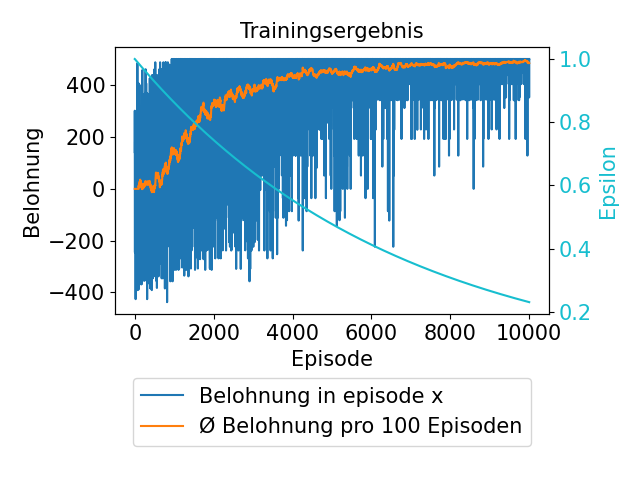
\includegraphics[width=\textwidth]{q_learning/figure_best.png}
        \caption{x-Achse zeigt die Episode, y-Achse zeigt die Belohnung. Eingezeichnet sind exakte Belohnung (blau), deren moving average (orange) und der Wert von $ \epsilon $ (türkis, Achse rechts) pro Episode.}
        \label{img:graphQBest}
    \end{subfigure}
    \begin{subfigure}[b]{0.49\textwidth}
        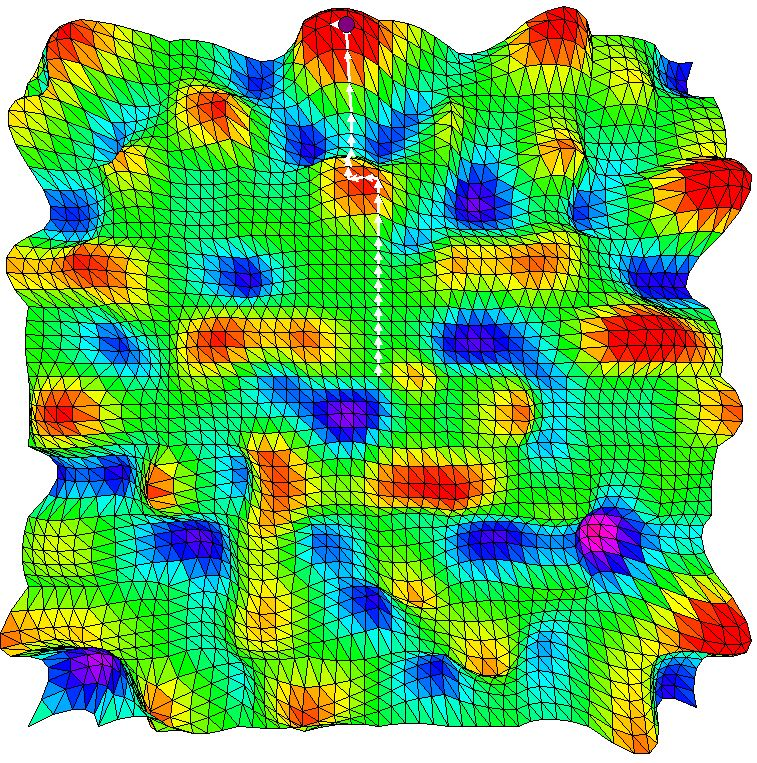
\includegraphics[width=\textwidth]{q_learning/terrain_path_best_white_3.JPG}
        \caption{Bester Pfad des Agenten nach dem Training}
        \label{img:pathQBest}
    \end{subfigure}
    \caption{Trainingsergebnisse des ersten Experiments}
\end{figure}

Eine weiter interessanter Wert ist die Anzahl der mit 0 belegten Einträge in der Q-table. Diese besitzen entweder zufällig den errechneten Q-value 0 oder wurden vom Agenten nicht berechnet. Da die meisten Einträge im 14-Stelligen Nachkommabereich liegen, ist ersteres relativ unwahrscheinlich und so lässt sich sagen, dass die Summe der mit 0 belegten Einträge ungefähr der Summe der nicht erkundeten Zustände entspricht. In Fall des aktuellen Experiments sind 850 der 10000 Einträge mit 0 belegt. Der Agent hat also ungefähr $ 91.5\% $ der Umgebung erkundet.

Dies ist nur ein einzelnes Experiment und hat natürlich keine statistische Aussagekraft. Es diente lediglich der Demonstration und der Erklärung der Visualisierung. Wir werden im Folgenden testen, welche Auswirkung die Verwendung der $ \epsilon $-greedy Strategie auf den Lernprozess hat.

\paragraph{Vergleich des Trainings mit und ohne $ \epsilon $-greedy Strategie}
Um eine aussagenkräftigere Datengrundlage zu erhalten, werden wir die folgenden Experimente jeweils 20 mal wiederholen. Diese Zahl hat sich als ein gutes Mittelmaß zwischen einer ausreichenden Menge an Daten für die Statistik und der Berechenbarkeit in zumutbarer Zeit erwiesen.

Die erste Experimentreihe erfolgt mit den gleichen Parametern wie im vorherigen Experiment. Für die zweite Experimentreihe setzen wir lediglich $ \epsilon $ auf 0. Das kommt dem Weglassen der $ \epsilon $-greedy Strategie gleich und bedeutet, dass der Agent in jedem Fall greedy agiert und die beste Aktion wählt. Dies soll die Notwendigkeit von $ \epsilon $ für ein besseres Trainingsergebnis zeigen.
\begin{figure}[H]
    \centering
    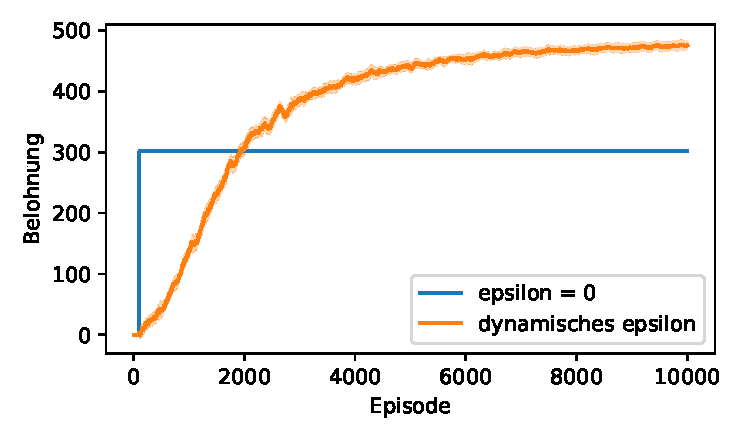
\includegraphics{q_learning/figure_epsilon_compare.pdf}
    \caption{Vergleich der Trainingsverläufe mit und ohne $ \epsilon $-greedy Strategie nach jeweils 20 Wiederholungen. Der Graph zeigt den moving average und dessen Standardabweichung pro Episode.} \label{img:graphQEpsComp}
\end{figure}
Die Achsen von Graph \ref{img:graphQEpsComp} sind bis auf das Fehlen der $ \epsilon $-Achse identisch mit dem aus \ref{img:graphQBest}. Die beiden Linien zeigen jeweils den Durchschnitt der moving average Werte aller 20 Experimentiterationen. Der leicht transparente Bereich um die Linien herum ist die Standartabweichung in der jeweiligen Episode.
Es lässt sich hier sehr deutlich erkennen, dass der Agent ohne eine Erkundungsstrategie wie $ \epsilon $-greedy (blaue Linie) zu Beginn einen relativ lukrativen Pfad findet, diesen aber dann auch nicht mehr verlässt, um andere Pfade zu erkunden und so immer die gleiche Belohnung bekommt. Er wird schließlich vom $ \epsilon $-greedy Agenten (orange Linie) überholt, da dieser seine Umgebung erkundet. Dieser erhält am Ende des Trainings wesentlich höhere Belohnungen.

Betrachten wir den Durchschnitt der Anzahl der mit 0 belegten Einträge der Q-tables beider Experimentreihen lässt sich abschätzen, dass der $ \epsilon $-greedy Agent im Schnitt $ 89.9\% $ der Umgebung erkundet hat, während es beim Agent ohne Erkundungsstrategie gerade einmal $ 1.1\% $ sind.

Dies zeigt, dass eine Erkundungsstrategie für den Erfolg des Agenten sehr wichtig ist.

\paragraph{Erkundungsstrategie codiert im Reward}
Für das nächste Experiment lassen wir der Agenten ebenfalls in jedem Zeitschritt greedy agieren. Diesmal erreichen wir dies, indem wir unabhängig vom aktuellen $ \epsilon $ immer die beste Aktion auswählen. Der Agent soll allein durch die Veränderung der Belohnung dazu gebracht werden, seine Umgebung besser zu erkunden und trotzdem einen möglichst hohen Punkt zu finden.

Wir modifizieren hierfür die nach jeder Aktion von der Umgebung erhaltene Belohnung wiefolgt:
\begin{minted}{python}
new_state, actual_reward, _ = environment.agent_perform_action(action)

reward = ((1 - exploration_rate) * actual_reward) - exploration_rate

sars = (state, action, reward, new_state)
buffer.append(sars)
\end{minted}
Die \mintinline{python}{exploration_rate} verhält sich hierbei genau so wie beim Experiment davor. Diese Formel soll bewirken, dass der Agent zu Beginn bei einer hohen \mintinline{python}{exploration_rate} alle besuchten Felder mit einem negativen Wert belegt, sodass er beim nächsten mal andere Felder besucht und so seine Umgebung erkundet. Nach und nach wird diese Belegung dann immer mehr mit den mittels korrekter Belohnungen ermittelten Q-values ersetzt, wodurch sich der Agent auf die besten Zustände einpendeln soll. Wir setzen die learning rate auf 1, damit der Agent nicht an den zu Beginn verfälschten Belohnungen festhält. Nach 50000 Episoden erhält man folgendes Ergebnis:
\begin{figure}[H]
    \centering
    \begin{subfigure}[b]{0.49\textwidth}
        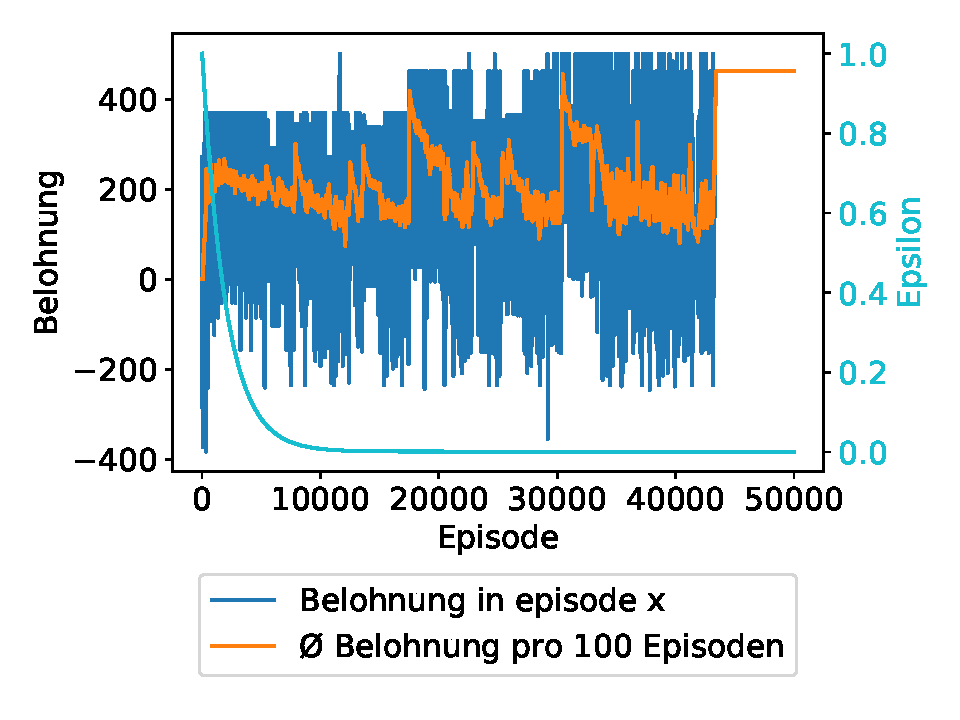
\includegraphics[width=\textwidth]{q_learning/figure_epsilon_in_reward_2.pdf}
        \caption{Graph so wie in \ref{img:graphQBest}}
        \label{img:graphQEpsInRew}
    \end{subfigure}
    \begin{subfigure}[b]{0.49\textwidth}
        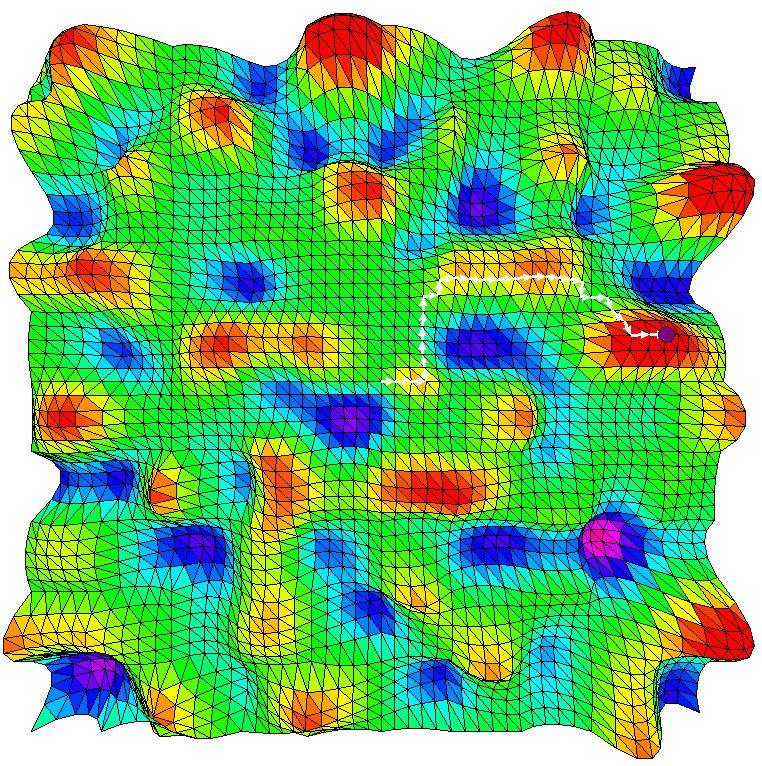
\includegraphics[width=\textwidth]{q_learning/terrain_epsilon_in_reward.JPG}
        \caption{Bester Pfad des Agenten nach dem Training}
        \label{img:pathQEpsInRew}
    \end{subfigure}
    \caption{Trainingsergebnisse mit Erkundungsstrategie codiert im Reward}
\end{figure}
Wichtig ist es an dieser Stelle zu erwähnen, dass der Graph \ref{img:graphQEpsInRew} die unverfälschte, von der Umgebung gelieferte Belohnung vor der Modifikation zeigt, da uns der tatsächliche Lernfortschritt des Agenten interessiert und man diesen sonst nicht mit den Ergebnissen anderen Experimente vergleichen könnte. Es fällt deutlich auf, dass der Lernprozess hier anders verläuft als in \ref{img:graphQBest}. Wir erhalten keine saubere Lernkurve. Trotzdem erreicht der Agent einen maximalen moving average von etwas über 462. Zum Vergleich: Der maximale moving average von \ref{img:graphQBest} liegt bei etwas über 497. Die Q-table dieses Experiments enthält 850 von 10000 mit Null belegte Einträge.

Abbildung \ref{img:pathQEpsInRew} zeigt den Pfad des Agenten bei Verwendung der erzeugten Q-table. Er findet zwar nicht den höchsten Punkt, erklimmt aber dennoch einen hohen Berg, welcher sich nicht in unmittelbarer Nähe des Startzustands befindet. Die Strategie hat also zur besseren Erkundung der Umgebung beigetragen.

Wiederholt man das Experiment 20 mal, so lässt sich der folgende Durchschnitt mit Standartabweichung berechnen:
\begin{figure}[H]
    \centering
    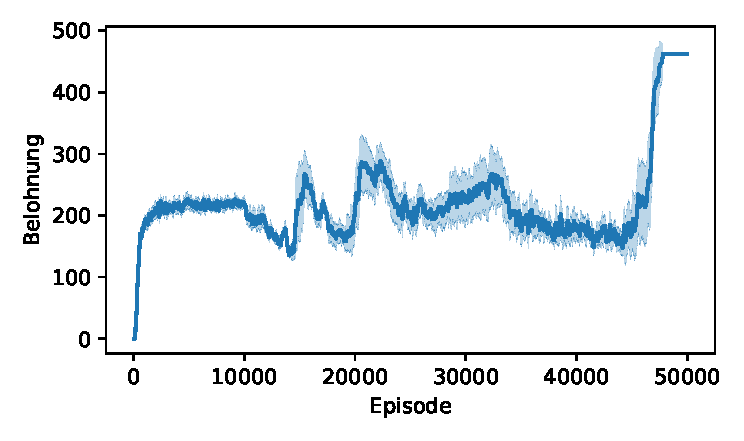
\includegraphics{q_learning/figure_epsilon_in_reward_mean.pdf}
    \caption{Trainingsergebnisse mit Erkundungsstrategie codiert im Reward nach 20 Wiederholungen. Graph so wie in \ref{img:graphQEpsComp}.} \label{img:graphQEpsInRewMean}
\end{figure}
Der Agent benötigt mit 50000 Episoden sehr lange, um seinen Höchstwert zu erreichen. Dieser scheint sich auch nach circa Episode 47 nicht mehr zu verändern, was vermutlich darauf zurückzuführen ist, dass der Agent immer greedy agiert und zu diesem Zeitpunkt kein besserer ihm bekannter Pfad mehr existiert. Verglichen mit dem Agenten ohne Erkundungsstrategie lässt sich festhalten, dass die Modifikation der Belohnung in diesem Fall eine höheren Ertrag sowie eine bessere Erkundung der Umgebung bewirkt hat. Diese Strategie dauert allerdings deutlich länger und liefert etwas weniger Ertrag als die klassische $ \epsilon $-greedy Strategie.
% \begin{minted}{python}
% params = Parameters(
%         num_episodes=100,
%         max_steps_per_episode=20,

%         learning_rate=0.5,
%         discount_rate=0.99,

%         start_exploration_rate=1,
%         max_exploration_rate=1,
%         min_exploration_rate=0.01,
%         exploration_decay_rate=0.1,

%         rewards_all_episodes=[],
%         max_rewards_all_episodes=[],
%     )
% \end{minted}

% https://github.com/simoninithomas/Deep_reinforcement_learning_Course/tree/master/Q%20learning/FrozenLake

% \begin{figure}[h]
%     \centering
%     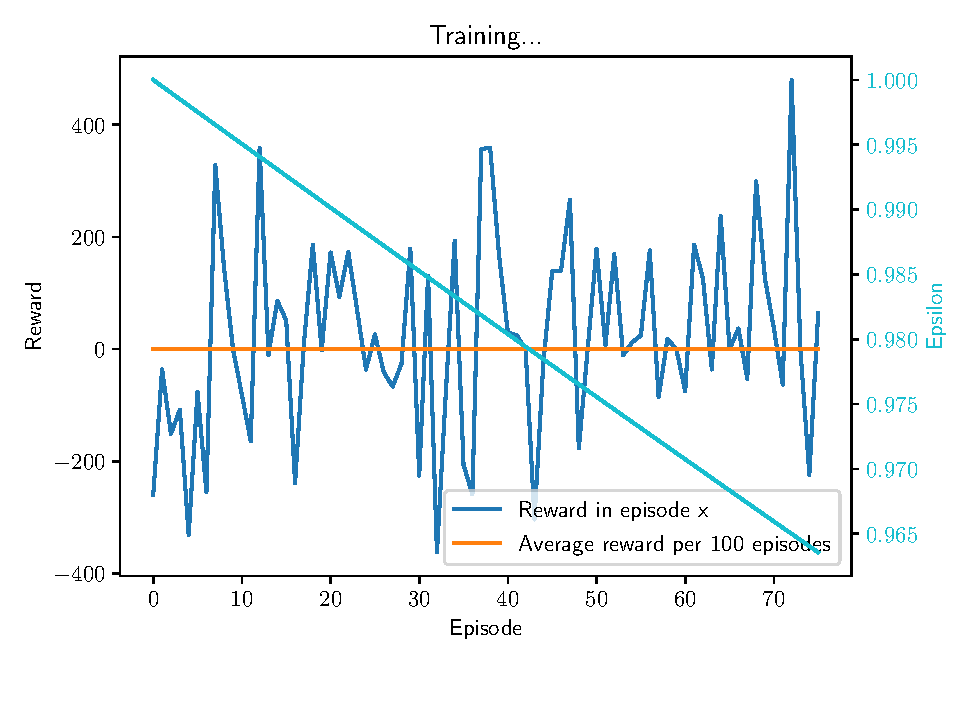
\includegraphics[width=\textwidth]{plot_test.pdf}
%     \caption{Visualisierung von zweidimensionaler Perlin Noise} \label{img:terrainMain}
% \end{figure}

% \begin{align}
%     \mathcal{F}(\theta) & = H(A|S,Z) - H(Z|S) + H(Z) \nonumber\\
%     & = H(A|S,Z) + E_{z \sim p(z), s \sim \pi(z)}(log\ p(z | s)) - E_{z \sim p(z)}(log\ p(z)) \label{eq:objective_2}\\
%     & \ge H(A|S,Z) + E_{z \sim p(z), s \sim \pi(z)}(log\ q_\phi(z | s) - log\ p(z)) \stackrel{\triangle}{=} \mathcal{G}(\theta, \phi) \nonumber
% \end{align}


% Grid, auf dem sich der Agent bewegen
% Perlin Noise
% 
% Color-coded: Rot ist hoch, blau ist tief
% 

%% Ziel des Agenten

%% Agent mit Q-Table

%% Agent mit Neuronalem Netz

%% Ergebnisse

% \begin{minted}{python}
%     import numpy as np
      
%     def incmatrix(genl1,genl2):
%         m = len(genl1)
%         n = len(genl2)
%         M = None #to become the incidence matrix
%         VT = np.zeros((n*m,1), int)  #dummy variable
      
%         #compute the bitwise xor matrix
%         M1 = bitxormatrix(genl1)
%         M2 = np.triu(bitxormatrix(genl2),1) 
      
%         for i in range(m-1):
%             for j in range(i+1, m):
%                 [r,c] = np.where(M2 == M1[i,j])
%                 for k in range(len(r)):
%                     VT[(i)*n + r[k]] = 1;
%                     VT[(i)*n + c[k]] = 1;
%                     VT[(j)*n + r[k]] = 1;
%                     VT[(j)*n + c[k]] = 1;
      
%                     if M is None:
%                         M = np.copy(VT)
%                     else:
%                         M = np.concatenate((M, VT), 1)
      
%                     VT = np.zeros((n*m,1), int)
      
%         return M
%     \end{minted}